% ---------------------------------------------------------------------------
% Results section (~1.5 pages in ACL format). Use in report/midway/main.tex:
%   % !TEX root = main.tex
% chktex-file 3
% chktex-file 8
% chktex-file 12
% chktex-file 13
% chktex-file 21
% chktex-file 24
% chktex-file 46
% Table 1 (single column) for the Results section. Passkey: standard prompt
% (test_passkey_v2_n50_*.json). Parameter counts are in the caption.

\begin{table}[t]
\centering
\footnotesize
\setlength{\tabcolsep}{2.4pt}
\begin{tabular}{@{}l rrr r rrr@{}}
\toprule
& \multicolumn{3}{c}{PPL $\downarrow$} & PK $\uparrow$ & \multicolumn{3}{c}{RULER $\uparrow$} \\
\cmidrule(lr){2-4}\cmidrule(lr){5-5}\cmidrule(lr){6-8}
Method & 4k & 8k & 16k & 16k & 4k & 8k & 16k \\
\midrule
Original     & \textbf{16.4} & 124.6 & 430.3 & 0 & \textbf{72.8} & 0.0 & 0.0 \\
PI ($\times 4$)   & 109.1 & 118.5 & 110.9 & 0 & 0.0 & 0.0 & 0.0 \\
YaRN, default     & 27.1 & 40.1 & 41.7 & 1 & 8.3 & 6.6 & 1.2 \\
YaRN, tuned       & 19.9 & 22.9 & 21.4 & 80 & 45.7 & 35.4 & 24.0 \\
\midrule
\multicolumn{8}{l}{\textit{Frequencies only, from $a{=}0$}} \\
\quad Shared      & 21.8 & 23.9 & 22.5 & 0 & 12.2 & 4.7 & 0.2 \\
\quad Per layer   & 20.0 & 21.3 & 19.5 & 0 & 39.3 & 21.9 & 1.3 \\
\quad Per head    & 20.7 & 21.8 & 19.7 & 0 & 5.8 & 0.8 & 0.0 \\
\multicolumn{8}{l}{\textit{Freq.\ + temperature, from $a{=}0$}} \\
\quad Shared      & 18.1 & 18.7 & 16.2 & \textbf{81} & 61.0 & 49.1 & 36.8 \\
\quad Per layer   & 17.9 & 18.4 & 16.0 & 1 & 59.9 & 43.7 & 33.3 \\
\quad Per head    & 18.7 & 19.4 & 17.2 & 0 & 24.5 & 21.3 & 5.9 \\
\multicolumn{8}{l}{\textit{Freq.\ + temperature, from YaRN}} \\
\quad Shared      & 17.3 & 17.8 & 15.4 & 80 & 61.4 & 49.0 & 36.2 \\
\quad Per layer   & 17.2 & 17.6 & 15.3 & 4 & 58.6 & 50.1 & 35.6 \\
\quad Per head    & 17.0 & \textbf{17.4} & \textbf{15.1} & 0 & 69.8 & \textbf{62.9} & \textbf{53.1} \\
\multicolumn{8}{l}{\textit{PoSE (4k text) + freq.\ + temp., from YaRN}} \\
\quad Shared      & 17.1 & 17.7 & 17.6 & 0 & 72.1 & 56.7 & 0.1 \\
\quad Per layer   & 17.3 & 17.8 & 18.6 & 0 & 65.8 & 47.5 & 0.0 \\
\quad Per head    & 17.1 & 17.6 & 16.5 & 0 & 59.1 & 43.1 & 1.1 \\
\bottomrule
\end{tabular}
\caption{Test results. Trainable parameters: 0 for the baselines; frequency scales
64 (shared), 1,024 (per layer) or 16,384 (per head), plus 512 for the temperature.
PPL: PG-19 perplexity. PK: passkey accuracy (\%) at 16k with the standard prompt, 250 prompts.
RULER: average over the 8 tasks (\%), 500 samples each.
PoSE from $a{=}0$ behaves the same as PoSE from YaRN.
Bold: best.}
\label{tab:main}
\end{table}
      Table 1 (full width); place it early in Experiments, between two paragraphs
%                              so it lands near its first mention (Intro and Results)
%   % ---------------------------------------------------------------------------
% Results section (~1.5 pages in ACL format). Use in report/midway/main.tex:
%   % !TEX root = main.tex
% chktex-file 3
% chktex-file 8
% chktex-file 12
% chktex-file 13
% chktex-file 21
% chktex-file 24
% chktex-file 46
% Table 1 (single column) for the Results section. Passkey: standard prompt
% (test_passkey_v2_n50_*.json). Parameter counts are in the caption.

\begin{table}[t]
\centering
\footnotesize
\setlength{\tabcolsep}{2.4pt}
\begin{tabular}{@{}l rrr r rrr@{}}
\toprule
& \multicolumn{3}{c}{PPL $\downarrow$} & PK $\uparrow$ & \multicolumn{3}{c}{RULER $\uparrow$} \\
\cmidrule(lr){2-4}\cmidrule(lr){5-5}\cmidrule(lr){6-8}
Method & 4k & 8k & 16k & 16k & 4k & 8k & 16k \\
\midrule
Original     & \textbf{16.4} & 124.6 & 430.3 & 0 & \textbf{72.8} & 0.0 & 0.0 \\
PI ($\times 4$)   & 109.1 & 118.5 & 110.9 & 0 & 0.0 & 0.0 & 0.0 \\
YaRN, default     & 27.1 & 40.1 & 41.7 & 1 & 8.3 & 6.6 & 1.2 \\
YaRN, tuned       & 19.9 & 22.9 & 21.4 & 80 & 45.7 & 35.4 & 24.0 \\
\midrule
\multicolumn{8}{l}{\textit{Frequencies only, from $a{=}0$}} \\
\quad Shared      & 21.8 & 23.9 & 22.5 & 0 & 12.2 & 4.7 & 0.2 \\
\quad Per layer   & 20.0 & 21.3 & 19.5 & 0 & 39.3 & 21.9 & 1.3 \\
\quad Per head    & 20.7 & 21.8 & 19.7 & 0 & 5.8 & 0.8 & 0.0 \\
\multicolumn{8}{l}{\textit{Freq.\ + temperature, from $a{=}0$}} \\
\quad Shared      & 18.1 & 18.7 & 16.2 & \textbf{81} & 61.0 & 49.1 & 36.8 \\
\quad Per layer   & 17.9 & 18.4 & 16.0 & 1 & 59.9 & 43.7 & 33.3 \\
\quad Per head    & 18.7 & 19.4 & 17.2 & 0 & 24.5 & 21.3 & 5.9 \\
\multicolumn{8}{l}{\textit{Freq.\ + temperature, from YaRN}} \\
\quad Shared      & 17.3 & 17.8 & 15.4 & 80 & 61.4 & 49.0 & 36.2 \\
\quad Per layer   & 17.2 & 17.6 & 15.3 & 4 & 58.6 & 50.1 & 35.6 \\
\quad Per head    & 17.0 & \textbf{17.4} & \textbf{15.1} & 0 & 69.8 & \textbf{62.9} & \textbf{53.1} \\
\multicolumn{8}{l}{\textit{PoSE (4k text) + freq.\ + temp., from YaRN}} \\
\quad Shared      & 17.1 & 17.7 & 17.6 & 0 & 72.1 & 56.7 & 0.1 \\
\quad Per layer   & 17.3 & 17.8 & 18.6 & 0 & 65.8 & 47.5 & 0.0 \\
\quad Per head    & 17.1 & 17.6 & 16.5 & 0 & 59.1 & 43.1 & 1.1 \\
\bottomrule
\end{tabular}
\caption{Test results. Trainable parameters: 0 for the baselines; frequency scales
64 (shared), 1,024 (per layer) or 16,384 (per head), plus 512 for the temperature.
PPL: PG-19 perplexity. PK: passkey accuracy (\%) at 16k with the standard prompt, 250 prompts.
RULER: average over the 8 tasks (\%), 500 samples each.
PoSE from $a{=}0$ behaves the same as PoSE from YaRN.
Bold: best.}
\label{tab:main}
\end{table}
      Table 1 (full width); place it early in Experiments, between two paragraphs
%                              so it lands near its first mention (Intro and Results)
%   % ---------------------------------------------------------------------------
% Results section (~1.5 pages in ACL format). Use in report/midway/main.tex:
%   % !TEX root = main.tex
% chktex-file 3
% chktex-file 8
% chktex-file 12
% chktex-file 13
% chktex-file 21
% chktex-file 24
% chktex-file 46
% Table 1 (single column) for the Results section. Passkey: standard prompt
% (test_passkey_v2_n50_*.json). Parameter counts are in the caption.

\begin{table}[t]
\centering
\footnotesize
\setlength{\tabcolsep}{2.4pt}
\begin{tabular}{@{}l rrr r rrr@{}}
\toprule
& \multicolumn{3}{c}{PPL $\downarrow$} & PK $\uparrow$ & \multicolumn{3}{c}{RULER $\uparrow$} \\
\cmidrule(lr){2-4}\cmidrule(lr){5-5}\cmidrule(lr){6-8}
Method & 4k & 8k & 16k & 16k & 4k & 8k & 16k \\
\midrule
Original     & \textbf{16.4} & 124.6 & 430.3 & 0 & \textbf{72.8} & 0.0 & 0.0 \\
PI ($\times 4$)   & 109.1 & 118.5 & 110.9 & 0 & 0.0 & 0.0 & 0.0 \\
YaRN, default     & 27.1 & 40.1 & 41.7 & 1 & 8.3 & 6.6 & 1.2 \\
YaRN, tuned       & 19.9 & 22.9 & 21.4 & 80 & 45.7 & 35.4 & 24.0 \\
\midrule
\multicolumn{8}{l}{\textit{Frequencies only, from $a{=}0$}} \\
\quad Shared      & 21.8 & 23.9 & 22.5 & 0 & 12.2 & 4.7 & 0.2 \\
\quad Per layer   & 20.0 & 21.3 & 19.5 & 0 & 39.3 & 21.9 & 1.3 \\
\quad Per head    & 20.7 & 21.8 & 19.7 & 0 & 5.8 & 0.8 & 0.0 \\
\multicolumn{8}{l}{\textit{Freq.\ + temperature, from $a{=}0$}} \\
\quad Shared      & 18.1 & 18.7 & 16.2 & \textbf{81} & 61.0 & 49.1 & 36.8 \\
\quad Per layer   & 17.9 & 18.4 & 16.0 & 1 & 59.9 & 43.7 & 33.3 \\
\quad Per head    & 18.7 & 19.4 & 17.2 & 0 & 24.5 & 21.3 & 5.9 \\
\multicolumn{8}{l}{\textit{Freq.\ + temperature, from YaRN}} \\
\quad Shared      & 17.3 & 17.8 & 15.4 & 80 & 61.4 & 49.0 & 36.2 \\
\quad Per layer   & 17.2 & 17.6 & 15.3 & 4 & 58.6 & 50.1 & 35.6 \\
\quad Per head    & 17.0 & \textbf{17.4} & \textbf{15.1} & 0 & 69.8 & \textbf{62.9} & \textbf{53.1} \\
\multicolumn{8}{l}{\textit{PoSE (4k text) + freq.\ + temp., from YaRN}} \\
\quad Shared      & 17.1 & 17.7 & 17.6 & 0 & 72.1 & 56.7 & 0.1 \\
\quad Per layer   & 17.3 & 17.8 & 18.6 & 0 & 65.8 & 47.5 & 0.0 \\
\quad Per head    & 17.1 & 17.6 & 16.5 & 0 & 59.1 & 43.1 & 1.1 \\
\bottomrule
\end{tabular}
\caption{Test results. Trainable parameters: 0 for the baselines; frequency scales
64 (shared), 1,024 (per layer) or 16,384 (per head), plus 512 for the temperature.
PPL: PG-19 perplexity. PK: passkey accuracy (\%) at 16k with the standard prompt, 250 prompts.
RULER: average over the 8 tasks (\%), 500 samples each.
PoSE from $a{=}0$ behaves the same as PoSE from YaRN.
Bold: best.}
\label{tab:main}
\end{table}
      Table 1 (full width); place it early in Experiments, between two paragraphs
%                              so it lands near its first mention (Intro and Results)
%   % ---------------------------------------------------------------------------
% Results section (~1.5 pages in ACL format). Use in report/midway/main.tex:
%   \input{results_table}      Table 1 (full width); place it early in Experiments, between two paragraphs
%                              so it lands near its first mention (Intro and Results)
%   \input{results}            in place of the old Results section + its table
%   \clearpage\appendix ... \input{results_appendix}   (figures moved out of the main text)
% Requires booktabs and graphicx (both loaded by main.tex).
% Numbers appear only in tables and figures. Sources: results/**/*.json, test split.
% Passkey uses the standard (Landmark-Attention) prompt, 750 prompts:
%   results/sweeps/*/test_passkey_v2_n50_*.json, results/passkey_n50/test_passkey_v2_n50_*.json
% ---------------------------------------------------------------------------

% Figures are copied into report/midway/figures/ (from Documentation/figures/) so the
% folder compiles on its own, e.g. on Overleaf.
\graphicspath{{figures/}}

\section{Results}
\label{sec:results}

Besides the baselines, we compare three families:
\emph{frequencies only} (RQ1, from $a{=}0$),
\emph{frequencies + temperature} (RQ1, from $a{=}0$ or from YaRN's values), and
the latter trained with \emph{PoSE} on 4k text only (RQ2).
Learning rates were chosen on the validation split; Table~\ref{tab:main} reports results on the separate test split, which was not used for any choices.
Tuned YaRN's settings come from a grid search scored with an earlier passkey
evaluation that had a bug and few prompts, so this baseline may be slightly
under-tuned.

\paragraph{RQ1: frequencies alone are not enough; the temperature is essential.}
Learning frequencies alone gives better long-text perplexity than tuned
YaRN, but retrieval collapses at 16k (Table~\ref{tab:main},
Figure~\ref{fig:ruler-length}).
We did not expect this. Perplexity rewards predicting the next word, which
mostly depends on the last few sentences, so a model can score well without
using text far back. Retrieval needs exactly that distant text.
Adding a learned temperature, with everything else unchanged, brings 16k
retrieval back (Appendix, Figure~\ref{fig:ablation}).
This is consistent with attention dilution (Introduction), which the
temperature counteracts.

\emph{From $a{=}0$}, every model with a temperature beats tuned YaRN on 16k
perplexity, and the shared and per-layer models also beat it on 16k RULER.
Per head does not: its many independent parameters need a good starting
point under our short training budget.
\emph{Starting from YaRN's values} (frequencies and temperature) is better
still. At every granularity it beats tuned YaRN on 16k perplexity and RULER,
and the matching $a{=}0$ model on 16k perplexity; on 16k RULER it wins by a
wide margin for per head and is on par for shared. It also trains far faster: these runs begin close to
their final loss, while runs from $a{=}0$ need hundreds of steps (Appendix,
Figure~\ref{fig:loss}).

\begin{figure}[!t]
  \centering
  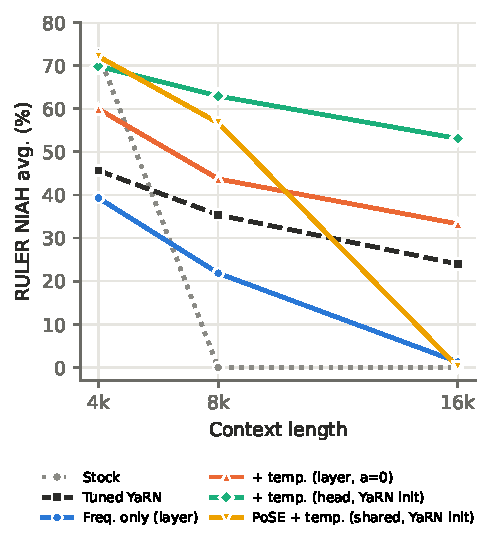
\includegraphics[width=\columnwidth]{fig_ruler_length.pdf}
  \caption{RULER score vs.\ input length for a representative model of each
  family. Frequencies only (blue) and PoSE (yellow) fall to zero at 16k;
  models with a learned temperature stay above tuned YaRN (dashed).}
  \label{fig:ruler-length}
\end{figure}

\paragraph{Cost at the native length.}
Only the models started from YaRN stay within one point of the original 4k
perplexity (Table~\ref{tab:main}), and they also recover much of the 4k RULER
score that tuned YaRN loses.

\paragraph{RQ2: short training text does not teach the temperature.}
As hypothesised, PoSE models trained on 4k text keep good perplexity and
retrieve well up to 8k, but fail at 16k retrieval at every granularity and
starting point, even though the temperature reads the skipped positions and
so sees 16k-like lengths: a 4k-token input never requires keeping attention
sharp over 16k real tokens.

\begin{table}[!t]
\centering
\small
\setlength{\tabcolsep}{3.5pt}
\begin{tabular}{ll rrrrr}
\toprule
& & \multicolumn{5}{c}{Depth of key} \\
\cmidrule(lr){3-7}
Model & Length & 0 & .25 & .5 & .75 & 1 \\
\midrule
Freq.\ only, layer & 8k  & 100 & 100 & 98 & 100 & 100 \\
                   & 16k & 0 & 0 & 0 & 0 & 0 \\
YaRN, tuned        & 16k & 88 & 90 & 76 & 52 & 96 \\
+ temp., shared    & 16k & 10 & 100 & 100 & 100 & 96 \\
\bottomrule
\end{tabular}
\caption{Passkey accuracy (\%) by depth of the key (0 = start of input,
1 = just before the question), 50 prompts per cell, standard prompt.
``+ temp., shared'' starts at $a{=}0$.}
\label{tab:depth}
\end{table}

\paragraph{Error analysis.}
\emph{Why do frequencies-only models fail at 16k?} Not because the key is too
far away: they fail at 16k even when the key sits just before the question,
while at 8k they succeed at every depth (Table~\ref{tab:depth}). Instead of
answering, they continue the filler text, with either passkey prompt.
A possible cause, not yet tested, is that some slow bands learned to rotate
faster than in pretraining (Appendix, Figure~\ref{fig:learned-a}), so distant
tokens can look close.

\emph{Which measure to trust?} Passkey and RULER rank the models
differently. The best model on RULER (per head, from YaRN) scores zero on 16k
passkey, while the shared models, which are weaker on RULER, pass it as often
as tuned YaRN does. Passkey hides the key in one sentence repeated thousands of
times, which is unlike real text; RULER hides it in real essays. We therefore
take RULER as the main measure. Perplexity does not predict retrieval either
(Appendix, Figure~\ref{fig:ppl-ruler}).

These results suggest that learning a temperature, taking it from YaRN when
training on short text (RQ2), and selecting models by retrieval rather than
perplexity would give better results. Our best model meets the success
criterion on perplexity and RULER at its current stage.
            in place of the old Results section + its table
%   \clearpage\appendix ... % !TEX root = main.tex
% chktex-file 3
% chktex-file 8
% chktex-file 12
% chktex-file 13
% chktex-file 21
% chktex-file 24
% chktex-file 46
% Appendix figures for results.tex. In report/midway/main.tex, after \appendix:
%   \section{Additional results}
%   \input{results_appendix}
% Figure paths are set by \graphicspath in results.tex.

\begin{figure}[!htbp]
  \centering
  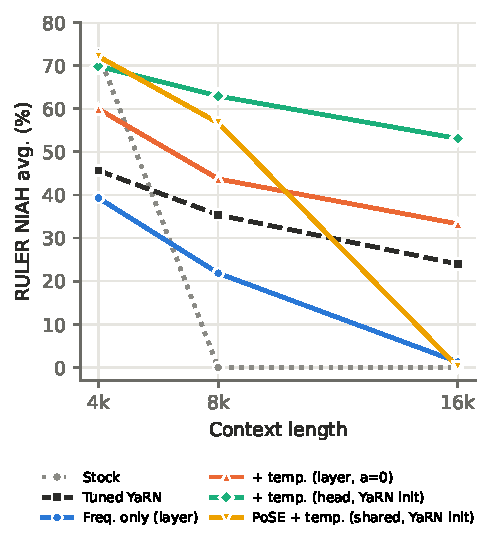
\includegraphics[width=\columnwidth]{fig_ruler_length.pdf}
  \caption{RULER score vs.\ input length for a representative model of each family. Frequencies only (blue) and PoSE (yellow) fall to zero at 16k; the models with a learned temperature shown here stay above tuned YaRN (dashed).}
  \label{fig:ruler-length}
\end{figure}

\begin{figure}[!htbp]
  \centering
  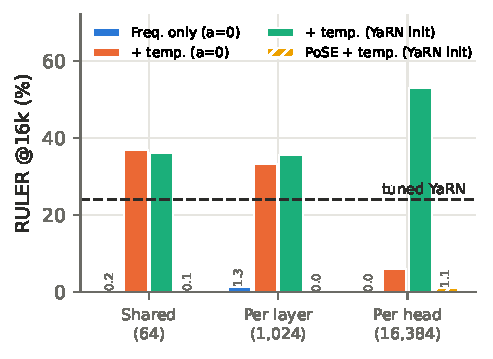
\includegraphics[width=\columnwidth]{fig_ablation_16k.pdf}
  \caption{RULER at 16k per granularity. Blue vs.\ orange differ only in the
  learned temperature; green starts both at YaRN; hatched yellow is PoSE
  (trained on 4k text). Dashed: tuned YaRN.}
  \label{fig:ablation}
\end{figure}

\begin{figure}[!htbp]
  \centering
  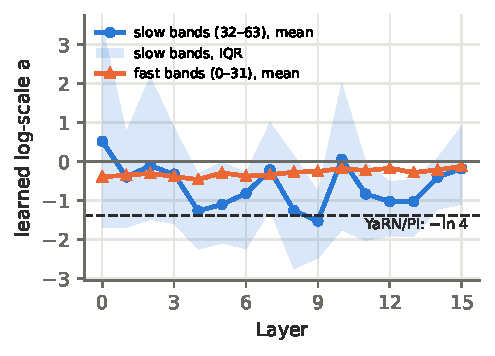
\includegraphics[width=\columnwidth]{fig_learned_a.pdf}
  \caption{Learned log frequency scales $a$ of the per-layer, frequencies-only
  model ($a<0$: slower rotation, $a=0$: unchanged). Line: mean over bands;
  shaded: middle 50\% of slow bands. Dashed: the single value YaRN and PI use
  for slow bands.}
  \label{fig:learned-a}
\end{figure}

\begin{figure}[!htbp]
  \centering
  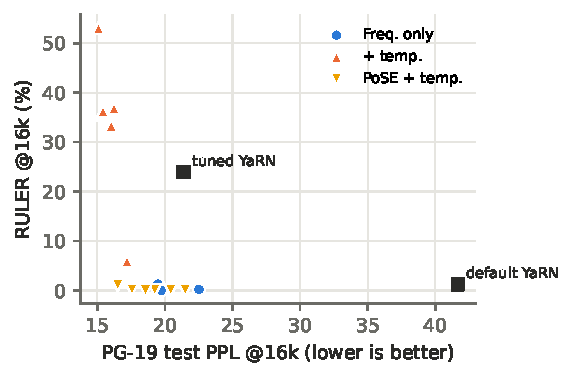
\includegraphics[width=\columnwidth]{fig_ppl_vs_ruler.pdf}
  \caption{PG-19 test perplexity vs.\ RULER score at 16k. Each marker is one
  trained model: frequencies only (blue), + temperature (orange), PoSE + temperature
  (yellow). The original model and PI are off the scale and not shown.}
  \label{fig:ppl-ruler}
\end{figure}

   (figures moved out of the main text)
% Requires booktabs and graphicx (both loaded by main.tex).
% Numbers appear only in tables and figures. Sources: results/**/*.json, test split.
% Passkey uses the standard (Landmark-Attention) prompt, 750 prompts:
%   results/sweeps/*/test_passkey_v2_n50_*.json, results/passkey_n50/test_passkey_v2_n50_*.json
% ---------------------------------------------------------------------------

% Figures are copied into report/midway/figures/ (from Documentation/figures/) so the
% folder compiles on its own, e.g. on Overleaf.
\graphicspath{{figures/}}

\section{Results}
\label{sec:results}

Besides the baselines, we compare three families:
\emph{frequencies only} (RQ1, from $a{=}0$),
\emph{frequencies + temperature} (RQ1, from $a{=}0$ or from YaRN's values), and
the latter trained with \emph{PoSE} on 4k text only (RQ2).
Learning rates were chosen on the validation split; Table~\ref{tab:main} reports results on the separate test split, which was not used for any choices.
Tuned YaRN's settings come from a grid search scored with an earlier passkey
evaluation that had a bug and few prompts, so this baseline may be slightly
under-tuned.

\paragraph{RQ1: frequencies alone are not enough; the temperature is essential.}
Learning frequencies alone gives better long-text perplexity than tuned
YaRN, but retrieval collapses at 16k (Table~\ref{tab:main},
Figure~\ref{fig:ruler-length}).
We did not expect this. Perplexity rewards predicting the next word, which
mostly depends on the last few sentences, so a model can score well without
using text far back. Retrieval needs exactly that distant text.
Adding a learned temperature, with everything else unchanged, brings 16k
retrieval back (Appendix, Figure~\ref{fig:ablation}).
This is consistent with attention dilution (Introduction), which the
temperature counteracts.

\emph{From $a{=}0$}, every model with a temperature beats tuned YaRN on 16k
perplexity, and the shared and per-layer models also beat it on 16k RULER.
Per head does not: its many independent parameters need a good starting
point under our short training budget.
\emph{Starting from YaRN's values} (frequencies and temperature) is better
still. At every granularity it beats tuned YaRN on 16k perplexity and RULER,
and the matching $a{=}0$ model on 16k perplexity; on 16k RULER it wins by a
wide margin for per head and is on par for shared. It also trains far faster: these runs begin close to
their final loss, while runs from $a{=}0$ need hundreds of steps (Appendix,
Figure~\ref{fig:loss}).

\begin{figure}[!t]
  \centering
  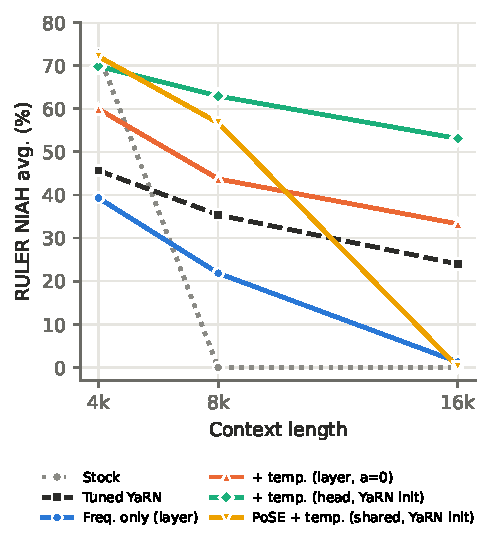
\includegraphics[width=\columnwidth]{fig_ruler_length.pdf}
  \caption{RULER score vs.\ input length for a representative model of each
  family. Frequencies only (blue) and PoSE (yellow) fall to zero at 16k;
  models with a learned temperature stay above tuned YaRN (dashed).}
  \label{fig:ruler-length}
\end{figure}

\paragraph{Cost at the native length.}
Only the models started from YaRN stay within one point of the original 4k
perplexity (Table~\ref{tab:main}), and they also recover much of the 4k RULER
score that tuned YaRN loses.

\paragraph{RQ2: short training text does not teach the temperature.}
As hypothesised, PoSE models trained on 4k text keep good perplexity and
retrieve well up to 8k, but fail at 16k retrieval at every granularity and
starting point, even though the temperature reads the skipped positions and
so sees 16k-like lengths: a 4k-token input never requires keeping attention
sharp over 16k real tokens.

\begin{table}[!t]
\centering
\small
\setlength{\tabcolsep}{3.5pt}
\begin{tabular}{ll rrrrr}
\toprule
& & \multicolumn{5}{c}{Depth of key} \\
\cmidrule(lr){3-7}
Model & Length & 0 & .25 & .5 & .75 & 1 \\
\midrule
Freq.\ only, layer & 8k  & 100 & 100 & 98 & 100 & 100 \\
                   & 16k & 0 & 0 & 0 & 0 & 0 \\
YaRN, tuned        & 16k & 88 & 90 & 76 & 52 & 96 \\
+ temp., shared    & 16k & 10 & 100 & 100 & 100 & 96 \\
\bottomrule
\end{tabular}
\caption{Passkey accuracy (\%) by depth of the key (0 = start of input,
1 = just before the question), 50 prompts per cell, standard prompt.
``+ temp., shared'' starts at $a{=}0$.}
\label{tab:depth}
\end{table}

\paragraph{Error analysis.}
\emph{Why do frequencies-only models fail at 16k?} Not because the key is too
far away: they fail at 16k even when the key sits just before the question,
while at 8k they succeed at every depth (Table~\ref{tab:depth}). Instead of
answering, they continue the filler text, with either passkey prompt.
A possible cause, not yet tested, is that some slow bands learned to rotate
faster than in pretraining (Appendix, Figure~\ref{fig:learned-a}), so distant
tokens can look close.

\emph{Which measure to trust?} Passkey and RULER rank the models
differently. The best model on RULER (per head, from YaRN) scores zero on 16k
passkey, while the shared models, which are weaker on RULER, pass it as often
as tuned YaRN does. Passkey hides the key in one sentence repeated thousands of
times, which is unlike real text; RULER hides it in real essays. We therefore
take RULER as the main measure. Perplexity does not predict retrieval either
(Appendix, Figure~\ref{fig:ppl-ruler}).

These results suggest that learning a temperature, taking it from YaRN when
training on short text (RQ2), and selecting models by retrieval rather than
perplexity would give better results. Our best model meets the success
criterion on perplexity and RULER at its current stage.
            in place of the old Results section + its table
%   \clearpage\appendix ... % !TEX root = main.tex
% chktex-file 3
% chktex-file 8
% chktex-file 12
% chktex-file 13
% chktex-file 21
% chktex-file 24
% chktex-file 46
% Appendix figures for results.tex. In report/midway/main.tex, after \appendix:
%   \section{Additional results}
%   % !TEX root = main.tex
% chktex-file 3
% chktex-file 8
% chktex-file 12
% chktex-file 13
% chktex-file 21
% chktex-file 24
% chktex-file 46
% Appendix figures for results.tex. In report/midway/main.tex, after \appendix:
%   \section{Additional results}
%   \input{results_appendix}
% Figure paths are set by \graphicspath in results.tex.

\begin{figure}[!htbp]
  \centering
  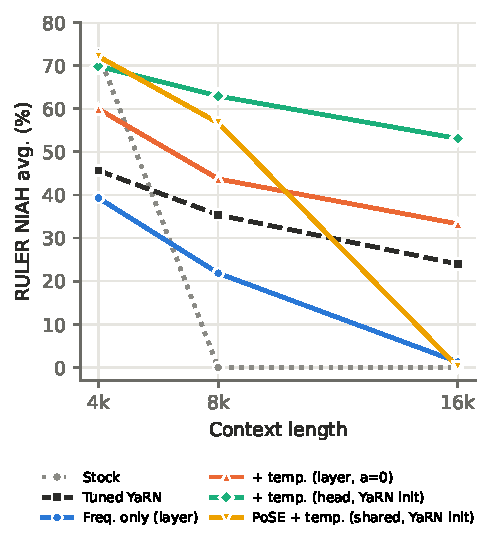
\includegraphics[width=\columnwidth]{fig_ruler_length.pdf}
  \caption{RULER score vs.\ input length for a representative model of each family. Frequencies only (blue) and PoSE (yellow) fall to zero at 16k; the models with a learned temperature shown here stay above tuned YaRN (dashed).}
  \label{fig:ruler-length}
\end{figure}

\begin{figure}[!htbp]
  \centering
  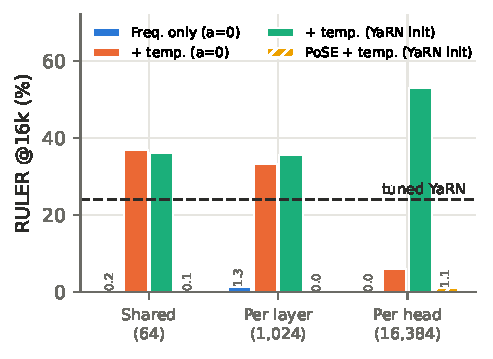
\includegraphics[width=\columnwidth]{fig_ablation_16k.pdf}
  \caption{RULER at 16k per granularity. Blue vs.\ orange differ only in the
  learned temperature; green starts both at YaRN; hatched yellow is PoSE
  (trained on 4k text). Dashed: tuned YaRN.}
  \label{fig:ablation}
\end{figure}

\begin{figure}[!htbp]
  \centering
  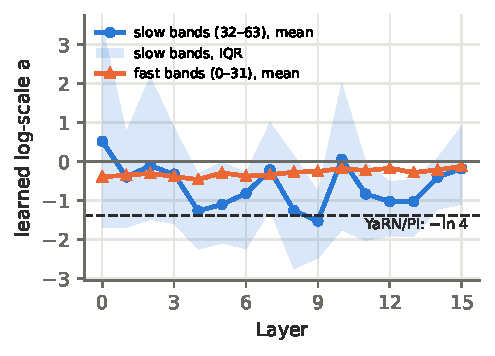
\includegraphics[width=\columnwidth]{fig_learned_a.pdf}
  \caption{Learned log frequency scales $a$ of the per-layer, frequencies-only
  model ($a<0$: slower rotation, $a=0$: unchanged). Line: mean over bands;
  shaded: middle 50\% of slow bands. Dashed: the single value YaRN and PI use
  for slow bands.}
  \label{fig:learned-a}
\end{figure}

\begin{figure}[!htbp]
  \centering
  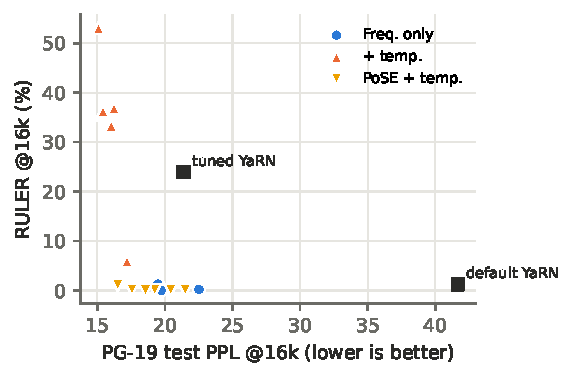
\includegraphics[width=\columnwidth]{fig_ppl_vs_ruler.pdf}
  \caption{PG-19 test perplexity vs.\ RULER score at 16k. Each marker is one
  trained model: frequencies only (blue), + temperature (orange), PoSE + temperature
  (yellow). The original model and PI are off the scale and not shown.}
  \label{fig:ppl-ruler}
\end{figure}


% Figure paths are set by \graphicspath in results.tex.

\begin{figure}[!htbp]
  \centering
  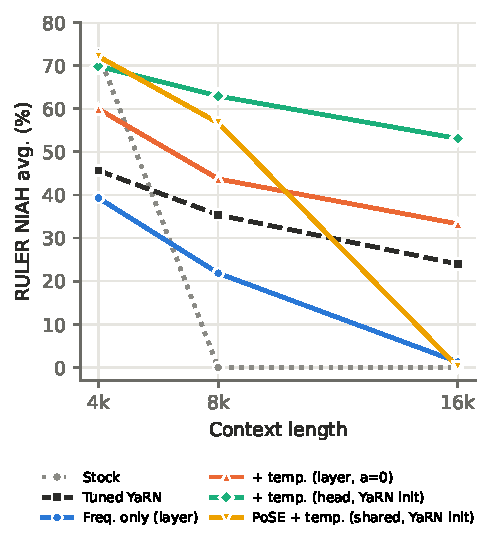
\includegraphics[width=\columnwidth]{fig_ruler_length.pdf}
  \caption{RULER score vs.\ input length for a representative model of each family. Frequencies only (blue) and PoSE (yellow) fall to zero at 16k; the models with a learned temperature shown here stay above tuned YaRN (dashed).}
  \label{fig:ruler-length}
\end{figure}

\begin{figure}[!htbp]
  \centering
  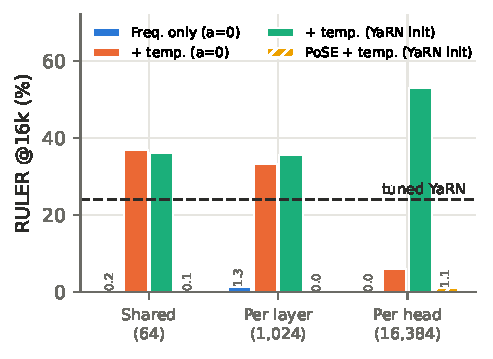
\includegraphics[width=\columnwidth]{fig_ablation_16k.pdf}
  \caption{RULER at 16k per granularity. Blue vs.\ orange differ only in the
  learned temperature; green starts both at YaRN; hatched yellow is PoSE
  (trained on 4k text). Dashed: tuned YaRN.}
  \label{fig:ablation}
\end{figure}

\begin{figure}[!htbp]
  \centering
  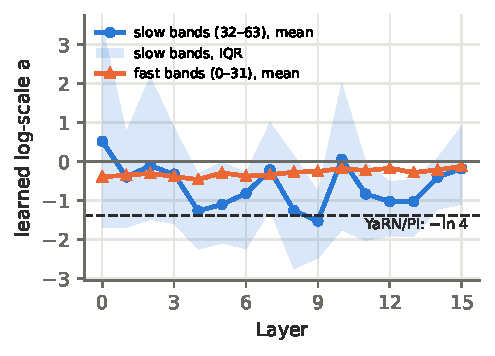
\includegraphics[width=\columnwidth]{fig_learned_a.pdf}
  \caption{Learned log frequency scales $a$ of the per-layer, frequencies-only
  model ($a<0$: slower rotation, $a=0$: unchanged). Line: mean over bands;
  shaded: middle 50\% of slow bands. Dashed: the single value YaRN and PI use
  for slow bands.}
  \label{fig:learned-a}
\end{figure}

\begin{figure}[!htbp]
  \centering
  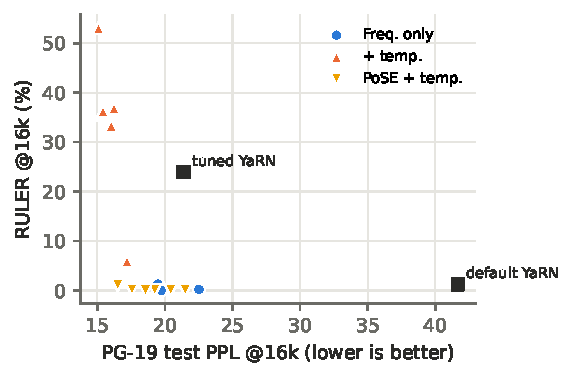
\includegraphics[width=\columnwidth]{fig_ppl_vs_ruler.pdf}
  \caption{PG-19 test perplexity vs.\ RULER score at 16k. Each marker is one
  trained model: frequencies only (blue), + temperature (orange), PoSE + temperature
  (yellow). The original model and PI are off the scale and not shown.}
  \label{fig:ppl-ruler}
\end{figure}

   (figures moved out of the main text)
% Requires booktabs and graphicx (both loaded by main.tex).
% Numbers appear only in tables and figures. Sources: results/**/*.json, test split.
% Passkey uses the standard (Landmark-Attention) prompt, 750 prompts:
%   results/sweeps/*/test_passkey_v2_n50_*.json, results/passkey_n50/test_passkey_v2_n50_*.json
% ---------------------------------------------------------------------------

% Figures are copied into report/midway/figures/ (from Documentation/figures/) so the
% folder compiles on its own, e.g. on Overleaf.
\graphicspath{{figures/}}

\section{Results}
\label{sec:results}

Besides the baselines, we compare three families:
\emph{frequencies only} (RQ1, from $a{=}0$),
\emph{frequencies + temperature} (RQ1, from $a{=}0$ or from YaRN's values), and
the latter trained with \emph{PoSE} on 4k text only (RQ2).
Learning rates were chosen on the validation split; Table~\ref{tab:main} reports results on the separate test split, which was not used for any choices.
Tuned YaRN's settings come from a grid search scored with an earlier passkey
evaluation that had a bug and few prompts, so this baseline may be slightly
under-tuned.

\paragraph{RQ1: frequencies alone are not enough; the temperature is essential.}
Learning frequencies alone gives better long-text perplexity than tuned
YaRN, but retrieval collapses at 16k (Table~\ref{tab:main},
Figure~\ref{fig:ruler-length}).
We did not expect this. Perplexity rewards predicting the next word, which
mostly depends on the last few sentences, so a model can score well without
using text far back. Retrieval needs exactly that distant text.
Adding a learned temperature, with everything else unchanged, brings 16k
retrieval back (Appendix, Figure~\ref{fig:ablation}).
This is consistent with attention dilution (Introduction), which the
temperature counteracts.

\emph{From $a{=}0$}, every model with a temperature beats tuned YaRN on 16k
perplexity, and the shared and per-layer models also beat it on 16k RULER.
Per head does not: its many independent parameters need a good starting
point under our short training budget.
\emph{Starting from YaRN's values} (frequencies and temperature) is better
still. At every granularity it beats tuned YaRN on 16k perplexity and RULER,
and the matching $a{=}0$ model on 16k perplexity; on 16k RULER it wins by a
wide margin for per head and is on par for shared. It also trains far faster: these runs begin close to
their final loss, while runs from $a{=}0$ need hundreds of steps (Appendix,
Figure~\ref{fig:loss}).

\begin{figure}[!t]
  \centering
  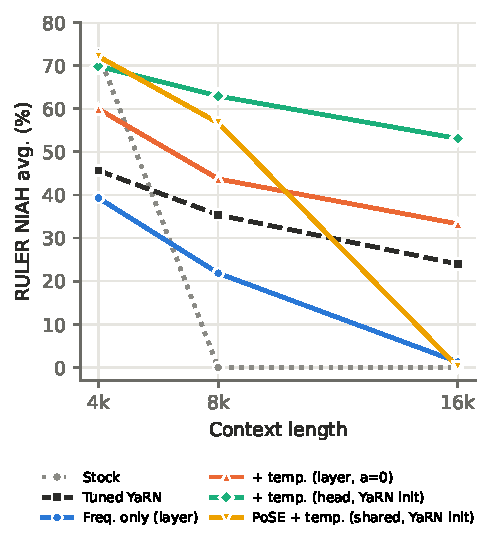
\includegraphics[width=\columnwidth]{fig_ruler_length.pdf}
  \caption{RULER score vs.\ input length for a representative model of each
  family. Frequencies only (blue) and PoSE (yellow) fall to zero at 16k;
  models with a learned temperature stay above tuned YaRN (dashed).}
  \label{fig:ruler-length}
\end{figure}

\paragraph{Cost at the native length.}
Only the models started from YaRN stay within one point of the original 4k
perplexity (Table~\ref{tab:main}), and they also recover much of the 4k RULER
score that tuned YaRN loses.

\paragraph{RQ2: short training text does not teach the temperature.}
As hypothesised, PoSE models trained on 4k text keep good perplexity and
retrieve well up to 8k, but fail at 16k retrieval at every granularity and
starting point, even though the temperature reads the skipped positions and
so sees 16k-like lengths: a 4k-token input never requires keeping attention
sharp over 16k real tokens.

\begin{table}[!t]
\centering
\small
\setlength{\tabcolsep}{3.5pt}
\begin{tabular}{ll rrrrr}
\toprule
& & \multicolumn{5}{c}{Depth of key} \\
\cmidrule(lr){3-7}
Model & Length & 0 & .25 & .5 & .75 & 1 \\
\midrule
Freq.\ only, layer & 8k  & 100 & 100 & 98 & 100 & 100 \\
                   & 16k & 0 & 0 & 0 & 0 & 0 \\
YaRN, tuned        & 16k & 88 & 90 & 76 & 52 & 96 \\
+ temp., shared    & 16k & 10 & 100 & 100 & 100 & 96 \\
\bottomrule
\end{tabular}
\caption{Passkey accuracy (\%) by depth of the key (0 = start of input,
1 = just before the question), 50 prompts per cell, standard prompt.
``+ temp., shared'' starts at $a{=}0$.}
\label{tab:depth}
\end{table}

\paragraph{Error analysis.}
\emph{Why do frequencies-only models fail at 16k?} Not because the key is too
far away: they fail at 16k even when the key sits just before the question,
while at 8k they succeed at every depth (Table~\ref{tab:depth}). Instead of
answering, they continue the filler text, with either passkey prompt.
A possible cause, not yet tested, is that some slow bands learned to rotate
faster than in pretraining (Appendix, Figure~\ref{fig:learned-a}), so distant
tokens can look close.

\emph{Which measure to trust?} Passkey and RULER rank the models
differently. The best model on RULER (per head, from YaRN) scores zero on 16k
passkey, while the shared models, which are weaker on RULER, pass it as often
as tuned YaRN does. Passkey hides the key in one sentence repeated thousands of
times, which is unlike real text; RULER hides it in real essays. We therefore
take RULER as the main measure. Perplexity does not predict retrieval either
(Appendix, Figure~\ref{fig:ppl-ruler}).

These results suggest that learning a temperature, taking it from YaRN when
training on short text (RQ2), and selecting models by retrieval rather than
perplexity would give better results. Our best model meets the success
criterion on perplexity and RULER at its current stage.
            in place of the old Results section + its table
%   \clearpage\appendix ... % !TEX root = main.tex
% chktex-file 3
% chktex-file 8
% chktex-file 12
% chktex-file 13
% chktex-file 21
% chktex-file 24
% chktex-file 46
% Appendix figures for results.tex. In report/midway/main.tex, after \appendix:
%   \section{Additional results}
%   % !TEX root = main.tex
% chktex-file 3
% chktex-file 8
% chktex-file 12
% chktex-file 13
% chktex-file 21
% chktex-file 24
% chktex-file 46
% Appendix figures for results.tex. In report/midway/main.tex, after \appendix:
%   \section{Additional results}
%   % !TEX root = main.tex
% chktex-file 3
% chktex-file 8
% chktex-file 12
% chktex-file 13
% chktex-file 21
% chktex-file 24
% chktex-file 46
% Appendix figures for results.tex. In report/midway/main.tex, after \appendix:
%   \section{Additional results}
%   \input{results_appendix}
% Figure paths are set by \graphicspath in results.tex.

\begin{figure}[!htbp]
  \centering
  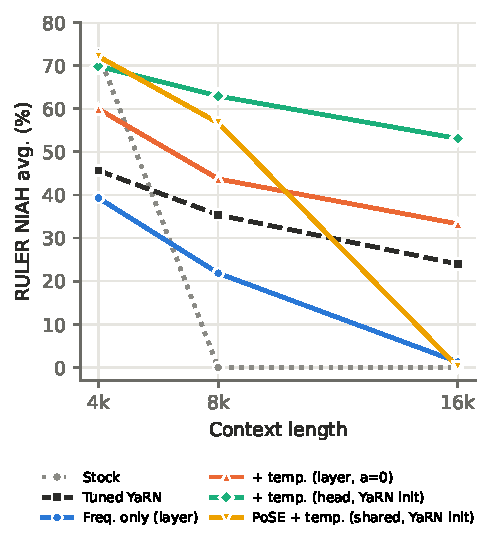
\includegraphics[width=\columnwidth]{fig_ruler_length.pdf}
  \caption{RULER score vs.\ input length for a representative model of each family. Frequencies only (blue) and PoSE (yellow) fall to zero at 16k; the models with a learned temperature shown here stay above tuned YaRN (dashed).}
  \label{fig:ruler-length}
\end{figure}

\begin{figure}[!htbp]
  \centering
  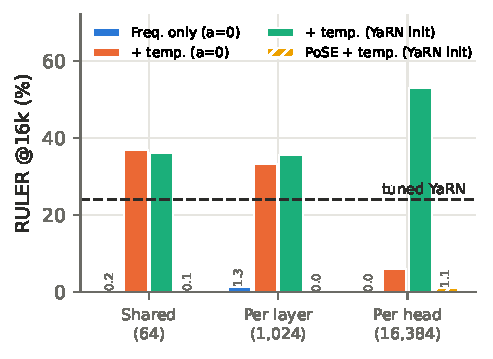
\includegraphics[width=\columnwidth]{fig_ablation_16k.pdf}
  \caption{RULER at 16k per granularity. Blue vs.\ orange differ only in the
  learned temperature; green starts both at YaRN; hatched yellow is PoSE
  (trained on 4k text). Dashed: tuned YaRN.}
  \label{fig:ablation}
\end{figure}

\begin{figure}[!htbp]
  \centering
  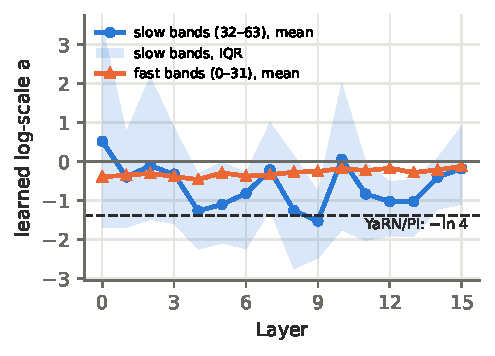
\includegraphics[width=\columnwidth]{fig_learned_a.pdf}
  \caption{Learned log frequency scales $a$ of the per-layer, frequencies-only
  model ($a<0$: slower rotation, $a=0$: unchanged). Line: mean over bands;
  shaded: middle 50\% of slow bands. Dashed: the single value YaRN and PI use
  for slow bands.}
  \label{fig:learned-a}
\end{figure}

\begin{figure}[!htbp]
  \centering
  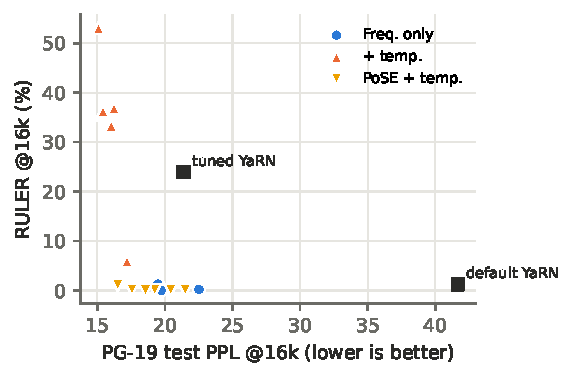
\includegraphics[width=\columnwidth]{fig_ppl_vs_ruler.pdf}
  \caption{PG-19 test perplexity vs.\ RULER score at 16k. Each marker is one
  trained model: frequencies only (blue), + temperature (orange), PoSE + temperature
  (yellow). The original model and PI are off the scale and not shown.}
  \label{fig:ppl-ruler}
\end{figure}


% Figure paths are set by \graphicspath in results.tex.

\begin{figure}[!htbp]
  \centering
  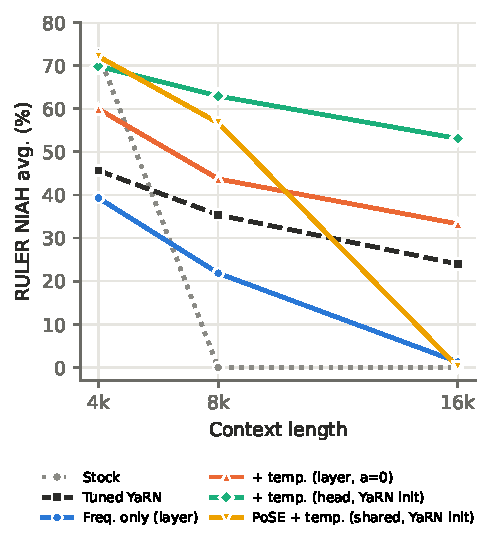
\includegraphics[width=\columnwidth]{fig_ruler_length.pdf}
  \caption{RULER score vs.\ input length for a representative model of each family. Frequencies only (blue) and PoSE (yellow) fall to zero at 16k; the models with a learned temperature shown here stay above tuned YaRN (dashed).}
  \label{fig:ruler-length}
\end{figure}

\begin{figure}[!htbp]
  \centering
  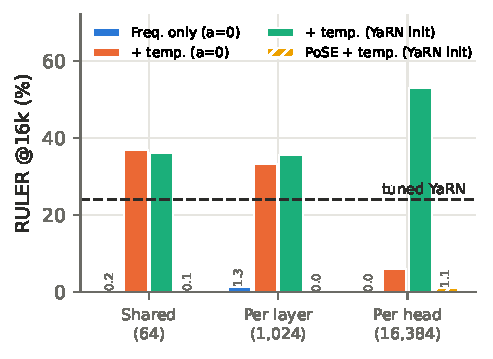
\includegraphics[width=\columnwidth]{fig_ablation_16k.pdf}
  \caption{RULER at 16k per granularity. Blue vs.\ orange differ only in the
  learned temperature; green starts both at YaRN; hatched yellow is PoSE
  (trained on 4k text). Dashed: tuned YaRN.}
  \label{fig:ablation}
\end{figure}

\begin{figure}[!htbp]
  \centering
  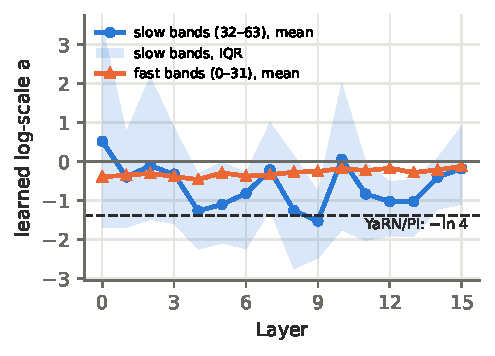
\includegraphics[width=\columnwidth]{fig_learned_a.pdf}
  \caption{Learned log frequency scales $a$ of the per-layer, frequencies-only
  model ($a<0$: slower rotation, $a=0$: unchanged). Line: mean over bands;
  shaded: middle 50\% of slow bands. Dashed: the single value YaRN and PI use
  for slow bands.}
  \label{fig:learned-a}
\end{figure}

\begin{figure}[!htbp]
  \centering
  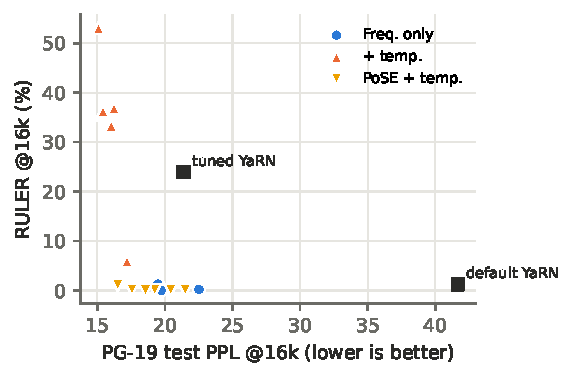
\includegraphics[width=\columnwidth]{fig_ppl_vs_ruler.pdf}
  \caption{PG-19 test perplexity vs.\ RULER score at 16k. Each marker is one
  trained model: frequencies only (blue), + temperature (orange), PoSE + temperature
  (yellow). The original model and PI are off the scale and not shown.}
  \label{fig:ppl-ruler}
\end{figure}


% Figure paths are set by \graphicspath in results.tex.

\begin{figure}[!htbp]
  \centering
  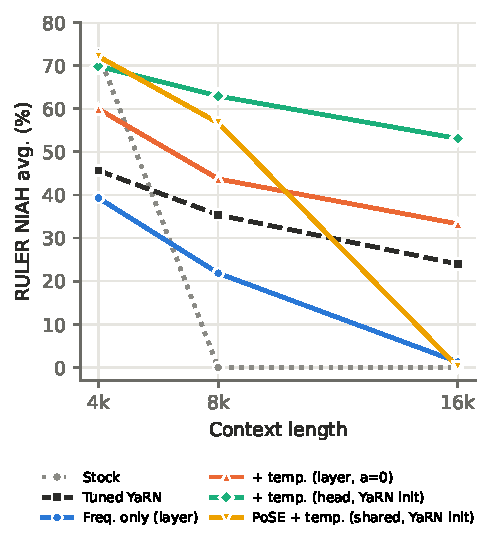
\includegraphics[width=\columnwidth]{fig_ruler_length.pdf}
  \caption{RULER score vs.\ input length for a representative model of each family. Frequencies only (blue) and PoSE (yellow) fall to zero at 16k; the models with a learned temperature shown here stay above tuned YaRN (dashed).}
  \label{fig:ruler-length}
\end{figure}

\begin{figure}[!htbp]
  \centering
  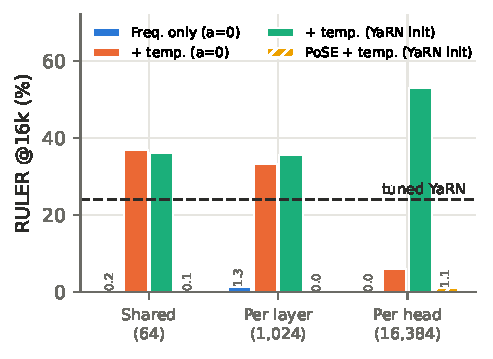
\includegraphics[width=\columnwidth]{fig_ablation_16k.pdf}
  \caption{RULER at 16k per granularity. Blue vs.\ orange differ only in the
  learned temperature; green starts both at YaRN; hatched yellow is PoSE
  (trained on 4k text). Dashed: tuned YaRN.}
  \label{fig:ablation}
\end{figure}

\begin{figure}[!htbp]
  \centering
  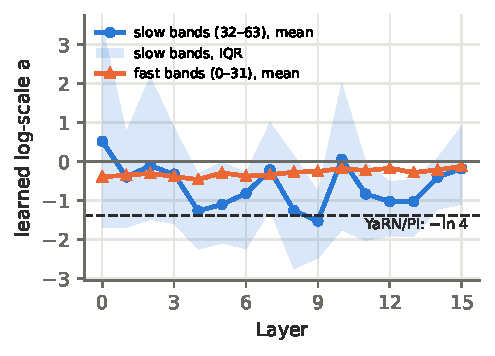
\includegraphics[width=\columnwidth]{fig_learned_a.pdf}
  \caption{Learned log frequency scales $a$ of the per-layer, frequencies-only
  model ($a<0$: slower rotation, $a=0$: unchanged). Line: mean over bands;
  shaded: middle 50\% of slow bands. Dashed: the single value YaRN and PI use
  for slow bands.}
  \label{fig:learned-a}
\end{figure}

\begin{figure}[!htbp]
  \centering
  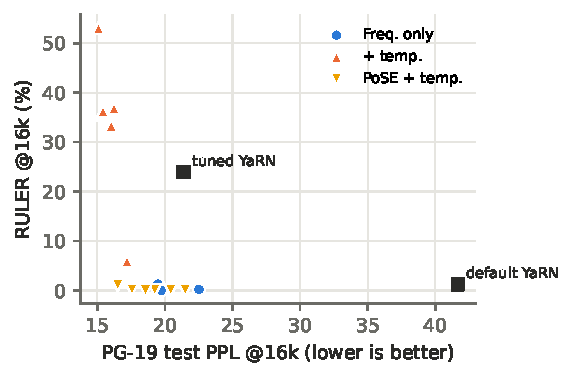
\includegraphics[width=\columnwidth]{fig_ppl_vs_ruler.pdf}
  \caption{PG-19 test perplexity vs.\ RULER score at 16k. Each marker is one
  trained model: frequencies only (blue), + temperature (orange), PoSE + temperature
  (yellow). The original model and PI are off the scale and not shown.}
  \label{fig:ppl-ruler}
\end{figure}

   (figures moved out of the main text)
% Requires booktabs and graphicx (both loaded by main.tex).
% Numbers appear only in tables and figures. Sources: results/**/*.json, test split.
% Passkey uses the standard (Landmark-Attention) prompt, 750 prompts:
%   results/sweeps/*/test_passkey_v2_n50_*.json, results/passkey_n50/test_passkey_v2_n50_*.json
% ---------------------------------------------------------------------------

% Figures are copied into report/midway/figures/ (from Documentation/figures/) so the
% folder compiles on its own, e.g. on Overleaf.
\graphicspath{{figures/}}

\section{Results}
\label{sec:results}

Besides the baselines, we compare three families:
\emph{frequencies only} (RQ1, from $a{=}0$),
\emph{frequencies + temperature} (RQ1, from $a{=}0$ or from YaRN's values), and
the latter trained with \emph{PoSE} on 4k text only (RQ2).
Learning rates were chosen on the validation split; Table~\ref{tab:main} reports results on the separate test split, which was not used for any choices.
Tuned YaRN's settings come from a grid search scored with an earlier passkey
evaluation that had a bug and few prompts, so this baseline may be slightly
under-tuned.

\paragraph{RQ1: frequencies alone are not enough; the temperature is essential.}
Learning frequencies alone gives better long-text perplexity than tuned
YaRN, but retrieval collapses at 16k (Table~\ref{tab:main},
Figure~\ref{fig:ruler-length}).
We did not expect this. Perplexity rewards predicting the next word, which
mostly depends on the last few sentences, so a model can score well without
using text far back. Retrieval needs exactly that distant text.
Adding a learned temperature, with everything else unchanged, brings 16k
retrieval back (Appendix, Figure~\ref{fig:ablation}).
This is consistent with attention dilution (Introduction), which the
temperature counteracts.

\emph{From $a{=}0$}, every model with a temperature beats tuned YaRN on 16k
perplexity, and the shared and per-layer models also beat it on 16k RULER.
Per head does not: its many independent parameters need a good starting
point under our short training budget.
\emph{Starting from YaRN's values} (frequencies and temperature) is better
still. At every granularity it beats tuned YaRN on 16k perplexity and RULER,
and the matching $a{=}0$ model on 16k perplexity; on 16k RULER it wins by a
wide margin for per head and is on par for shared. It also trains far faster: these runs begin close to
their final loss, while runs from $a{=}0$ need hundreds of steps (Appendix,
Figure~\ref{fig:loss}).

\begin{figure}[!t]
  \centering
  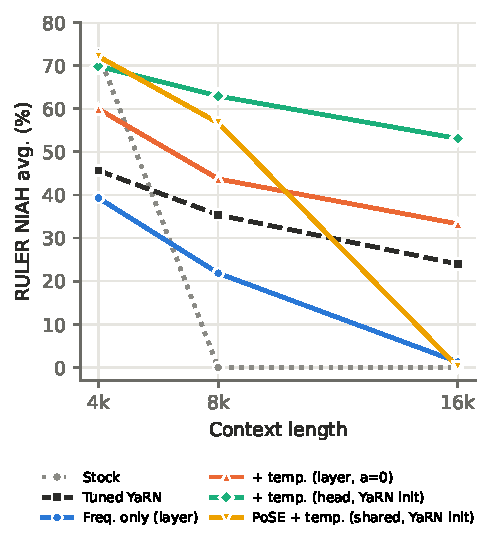
\includegraphics[width=\columnwidth]{fig_ruler_length.pdf}
  \caption{RULER score vs.\ input length for a representative model of each
  family. Frequencies only (blue) and PoSE (yellow) fall to zero at 16k;
  models with a learned temperature stay above tuned YaRN (dashed).}
  \label{fig:ruler-length}
\end{figure}

\paragraph{Cost at the native length.}
Only the models started from YaRN stay within one point of the original 4k
perplexity (Table~\ref{tab:main}), and they also recover much of the 4k RULER
score that tuned YaRN loses.

\paragraph{RQ2: short training text does not teach the temperature.}
As hypothesised, PoSE models trained on 4k text keep good perplexity and
retrieve well up to 8k, but fail at 16k retrieval at every granularity and
starting point, even though the temperature reads the skipped positions and
so sees 16k-like lengths: a 4k-token input never requires keeping attention
sharp over 16k real tokens.

\begin{table}[!t]
\centering
\small
\setlength{\tabcolsep}{3.5pt}
\begin{tabular}{ll rrrrr}
\toprule
& & \multicolumn{5}{c}{Depth of key} \\
\cmidrule(lr){3-7}
Model & Length & 0 & .25 & .5 & .75 & 1 \\
\midrule
Freq.\ only, layer & 8k  & 100 & 100 & 98 & 100 & 100 \\
                   & 16k & 0 & 0 & 0 & 0 & 0 \\
YaRN, tuned        & 16k & 88 & 90 & 76 & 52 & 96 \\
+ temp., shared    & 16k & 10 & 100 & 100 & 100 & 96 \\
\bottomrule
\end{tabular}
\caption{Passkey accuracy (\%) by depth of the key (0 = start of input,
1 = just before the question), 50 prompts per cell, standard prompt.
``+ temp., shared'' starts at $a{=}0$.}
\label{tab:depth}
\end{table}

\paragraph{Error analysis.}
\emph{Why do frequencies-only models fail at 16k?} Not because the key is too
far away: they fail at 16k even when the key sits just before the question,
while at 8k they succeed at every depth (Table~\ref{tab:depth}). Instead of
answering, they continue the filler text, with either passkey prompt.
A possible cause, not yet tested, is that some slow bands learned to rotate
faster than in pretraining (Appendix, Figure~\ref{fig:learned-a}), so distant
tokens can look close.

\emph{Which measure to trust?} Passkey and RULER rank the models
differently. The best model on RULER (per head, from YaRN) scores zero on 16k
passkey, while the shared models, which are weaker on RULER, pass it as often
as tuned YaRN does. Passkey hides the key in one sentence repeated thousands of
times, which is unlike real text; RULER hides it in real essays. We therefore
take RULER as the main measure. Perplexity does not predict retrieval either
(Appendix, Figure~\ref{fig:ppl-ruler}).

These results suggest that learning a temperature, taking it from YaRN when
training on short text (RQ2), and selecting models by retrieval rather than
perplexity would give better results. Our best model meets the success
criterion on perplexity and RULER at its current stage.
